\documentclass{article}
\usepackage[margin=1in]{geometry}
\usepackage{amsmath,amsthm,amssymb}
\usepackage{bbm,enumerate,mathtools}
\usepackage{tikz,pgfplots}
\usepackage{chessboard}
\usepackage[hidelinks]{hyperref}
\usepackage{multicol} % Problem 35
\usepackage{xstring} % Difficulty command
\usetikzlibrary{shapes.geometric}

\newenvironment{question}{\begin{trivlist}\item[\textbf{Question.}]}{\end{trivlist}}
\newenvironment{note}{\begin{trivlist}\item[\textbf{Note.}]}{\end{trivlist}}
\newenvironment{references}{\begin{trivlist}\item[\textbf{References.}]}{\end{trivlist}}
\newenvironment{related}{\begin{trivlist}\item[\textbf{Related.}]\end{trivlist}\begin{enumerate}}{\end{enumerate}}

\newcommand\score[1]{
\pgfmathsetmacro\pgfxa{#1+1}
\tikzstyle{scorestars}=[
  star,
  star points=5,
  star point ratio=2.25,
  draw,
  inner sep=3pt,
  anchor=outer point 5
]
  \begin{tikzpicture}[baseline]
    \draw[opacity=0] (0,-0.5) rectangle (0,0.2); % Workaround for whitespace at the bottom.
    \foreach \i in {1,...,4} {
      \pgfmathparse{(\i<=#1?"yellow":"gray")}
      \edef\starcolor{\pgfmathresult}
      \draw (\i*4.5ex,0) node[name=star\i,scorestars,fill=\starcolor]  {};
    }
  \end{tikzpicture}
}

\newcommand{\difficulty}[1]{%
  \IfEqCase{#1}{%
      {1}{
        
\begin{tikzpicture}[scale=0.7, baseline=0.9mm]%
          \definecolor{slopegreen}{rgb}{0.0, 0.5, 0.0}%
          \fill[slopegreen] (0.5,0.5) circle (0.5);%
        \end{tikzpicture}%
      }%
      {2}{
        
\begin{tikzpicture}[scale=0.7, baseline=0.9mm]%
          \definecolor{slopeblue}{rgb}{0.0, 0.44, 1.00}
          \fill[slopeblue] (0,0) rectangle (1,1);%
        \end{tikzpicture}%
      }%
      {3}{
\begin{tikzpicture}[scale=0.7, baseline=0.9mm]\fill (0,0.5)--(0.5, 0)--(1,0.5)--(0.5,1)--cycle; \end{tikzpicture}}%
      {4}{
\begin{tikzpicture}[scale=0.7, baseline=0.9mm]\fill (0.25,0)--(0,0.5)--(0.25,1)--(0.5,0.5)--cycle; \fill (0.75,0)--(0.5,0.5)--(0.75,1)--(1,0.5)--cycle;\end{tikzpicture}}%
      % you can add more cases here as desired
  }[\PackageError{difficulty}{Undefined difficulty level: #1}{}]%
}%
\newcommand{\rating}[2]{\difficulty{#1}\\\score{#2}\\}


\begin{document}
\rating{4}{2}
Consider convex polygons with integer coordinates. The notion of a best
Diophantine approximation can be generalized to equilateral triangles by
saying that a triangle is a better diophantine approximation if
the ratio of the largest side to the smallest side is less than the ratio of
any other triangle with smaller perimeter.
\begin{figure}[ht!]
  \centering
  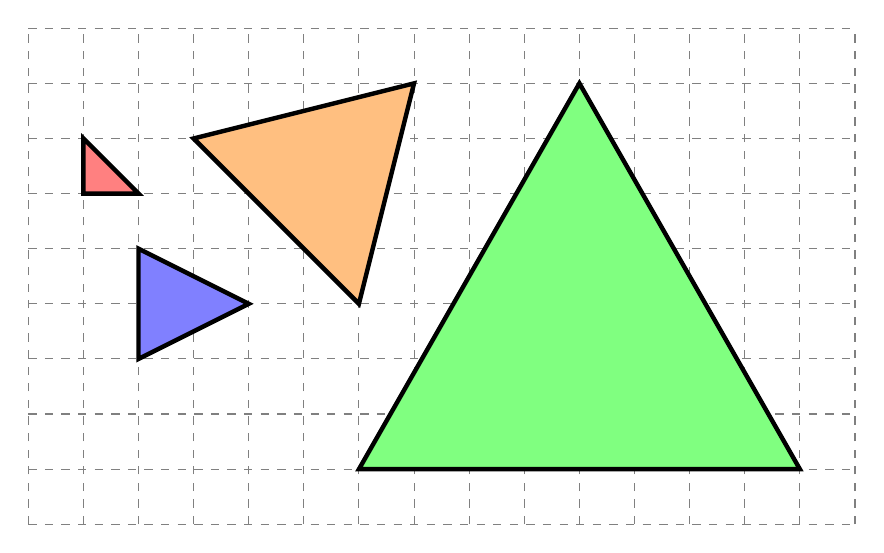
\begin{tikzpicture}[scale=0.7]
    \draw[gray, dashed] (0,0) grid (15,9);
    \draw[ultra thick, fill=red!50] (1,6)--(2,6)--(1,7)--cycle;
    \draw[ultra thick, fill=blue!50] (2,5)--(2,3)--(4,4)--cycle;
    \draw[ultra thick, fill=orange!50] (6,4)--(3,7)--(7,8)--cycle;
    \draw[ultra thick, fill=green!50] (6,1)--(14,1)--(10,8)--cycle;
  \end{tikzpicture}
  \caption{
    Four best (?) Diophantine approximations of an equilateral triangle.
    The red triangle has a ratio of $\sqrt{2/1} \approx 1.41$,
    the blue has a ratio of $\sqrt{5/4} \approx 1.118$,
    the orange has a ratio of $\sqrt{18/17} \approx 1.029$, and
    the green has a ratio of $\sqrt{64/63} \approx 1.008$.
  }
\end{figure}
\begin{question}
  What is the growth of the perimeter of the $k$-th best Diophantine
  approximation of an equilateral triangle as a function of $k$?
\end{question}

\begin{related}
  \item How can this be generalized in a reasonable way to regular $n$-gons?
    (Just looking at side lengths isn't enough---angles can behave badly.)
  \item What if this is done on tetrahedra?
\end{related}
\begin{references}
  \item \url{https://math.stackexchange.com/q/2251555/121988}
  \item \url{https://en.wikipedia.org/wiki/Near-miss_Johnson_solid}
\end{references}
\end{document}
